\documentclass[12pt]{article}
\usepackage{graphicx}
\usepackage[none]{hyphenat}
\usepackage{float}
\usepackage{tabularx}
\usepackage{longtable}
\usepackage{adjustbox}

% Title.
\title{Lab 8: Multiple String Detector}

% Author
\author{Mayank Gupta \\ Roll Number 210101002 \\}

%Date
\date{October 08, 2022}

% begin the document.
\begin{document}

	% make a title page.
	\maketitle

	% section 1: overview.
	\section{Overview of the experiment}
	
	\subsection{Purpose}
	
	The Multiple String Detector can be used to detect a sub sequence for a given sequence of letters. It uses Behavourial modelling in determining if the subsequence is present or not.
	Reset bit specifies the initial state and takes the operation back at the first step.
	
	This experiment helped us to understand Finite State Machines, their designing and usage in generating a sequence of bits using only clock and reset bits. It uses  Mealy type FSM, for which the output is a function of the current state and inputs.
	
	It helped in designing Finite State Machines by programming it on a hardware description language.
	
	\subsection{Procedure of the experiment}
	
	First, the logic of the clock processes was determined using the given code. Three processes were defined for the three different words: ``run'', ``cry'' and ``broom''.
	The present and the next state were defined for all these three processes. Three output signals were used for all the three processes.
	
	
	The main VHDL file was made, adding all necessary libraries, using the DUT, Gates, Testbench and Toplevel file for Scanchain sent to the students. The entities and architecture consisting of processes for clock and the three processes for the three words were made.
	Output process was also added in the architecture based on different states.
	
	Required files like Testbench and tracefile were added to the project. The gates were seen in the RTL viewer. 
	
	The waveform could be seen in Modelsim, and its correctness was verified using the generic testbench and given tracefile.

	The XEN10 board was then tested with the given .svf file.
	
	The .svf file was then uploaded on the board and then the output file was received using the scan application to check for success.
	
	\subsection{Organization of the report}
	
	The report contains the various entities, architectures and the components in the architecture used. It contains the truth tables and screenshots of the waveform in RTL simulation.
	
	% section 2: setup/approach.
	\section{Approach to the assignment}

	First all the libraries were included. Following that the entity was made. Then the architecture was setup along with the required components.

	The entity used for the Multiple String Detector is:
	\begin{verbatim}
		entity word_detection is
			port( inp:in std_logic_vector(4 downto 0);
			reset,clock:in std_logic;
			outp: out std_logic);
		end word_detection;


	\end{verbatim}

	\noindent The architecture along with all the functions used for the Multiple String Detector is:
	\begin{verbatim}
	architecture bhv of word_detection is
		type state is (rst, s1, s2, s3, s4, s5, s6, s7, s8,s9, s10, s11); 
		signal y_present1,y_next1: state:=rst;
		signal y_present2,y_next2: state:=rst;
		signal y_present3,y_next3: state:=rst;
		signal outp1, outp2, outp3: std_logic;
		begin
		clock_proc:process(clock,reset)
		begin
		if(clock='1' and clock' event) then
			if(reset='1') then
				y_present1<= rst;
				y_present2<= rst;
				y_present3<= rst;

			else
				y_present1<=y_next1;
				y_present2<=y_next2;
				y_present3<=y_next3;
			
			end if;
		end if;
		end process;
		state_transition_proc1:process(inp,y_present1)
		begin
			case y_present1 is
				when rst=>
					if(unsigned(inp)=18) then 
						y_next1<= s1;
						
					else
						y_next1<=rst;
					end if;
					
				when s1=>
					if (unsigned(inp)=21) then
						y_next1<= s2;
						
					else
						y_next1<=s1;
					end if;
					
				when s2=>
					if (unsigned(inp)=14) then
						y_next1<= s3;
						
					else
						y_next1<=s2;
					end if;
					
				when s3=>
					if(unsigned(inp)=18) then 
						y_next1<= s1;
						
					else
						y_next1<=rst;
					end if;
					
				when others=>
					
				
				end case;
				
			end process state_transition_proc1;
			
		state_transition_proc2:process(inp,y_present2)
		begin

			case y_present2 is
				when rst=>
					if(unsigned(inp)=3) then 
						y_next2<= s4;
						
					else
						y_next2<=rst;
					end if;
					
				when s4=>
					if (unsigned(inp)=18) then
						y_next2<= s5;
						
					else
						y_next2<=s4;
					end if;
					
				when s5=>
					if (unsigned(inp)=25) then
						y_next2<= s6;
						
					else
						y_next2<=s5;
					end if;
					
				when s6=>
					if(unsigned(inp)=3) then
						y_next2<= s4;
						
					else
						y_next2<=rst;
					end if;
					
				when others=>
				
				end case;
			end process state_transition_proc2;
			
		state_transition_proc3:process(inp,y_present3)
		begin
			
			
			case y_present3 is
				when rst=>
					if(unsigned(inp)=2) then
						y_next3<= s7;
						
					else
						y_next3<=rst;
					end if;
					
				when s7=>
					if (unsigned(inp)=18) then
						y_next3<= s8;
						
					else
						y_next3<=s7;
					end if;
					
				when s8=>
					if (unsigned(inp)=15) then
						y_next3<= s9;
						
					else
						y_next3<=s8;
					end if;
					
				when s9=>
					if (unsigned(inp)=15) then
						y_next3<= s10;
						
					else
						y_next3<=s9;
					end if;
					
				when s10=>
					if (unsigned(inp)=13) then
						y_next3<= s11;
						
					else
						y_next3<=s10;
					end if;
					
				when s11=>
					if(unsigned(inp)=2) then
						y_next3<= s7;
						
					else
						y_next3<=rst;
					end if;
					
				when others=>
				end case;
			end process state_transition_proc3;
			

				
		output_proc1:process(y_present1, inp) 
		begin
			case y_present1 is
				when rst =>
					outp1<='0';
				when s1=>
					outp1<='0';
				when s2=>
					if (unsigned(inp)=14) then
						outp1<='1';
					else
						outp1<='0';
					end if;
				when s3=>
					outp1<='0';
				when others =>
					outp1<='0';
				
			end case;
		end process output_proc1;
		output_proc2:process(y_present2, inp) 

		begin
			case y_present2 is
				when rst=>
					outp2<='0';
				when s4=>
					outp2<='0';
				when s5=>
					if (unsigned(inp)=25) then
						outp2<='1';
					else
						outp2<='0';
					end if;
				when s6=>
					outp2<='0';
				when others=>
					outp2<='0';
			end case;
		end process output_proc2;
		output_proc3:process(y_present3, inp) 
		begin
			case y_present3 is
				when rst=>
					outp3<='0';
				when s7=>
					outp3<='0';
				when s8=>
					outp3<='0';
				when s9=>
					outp3<='0';
				when s10=>
					if (unsigned(inp)=13) then
						outp3<='1';
					else
						outp3<='0';
					end if;
				when s11=>
					outp3<='0';
				when others=>
					outp3<='0';
			end case;
		end process output_proc3;
		outp<= outp1 or outp2 or outp3;
		end bhv;


	\end{verbatim}

	\pagebreak
	\section{Observations}

	% Tables.
	
	Truth table for the Multiple String Detector
	%\begin{table}[H]
		

		
		\begin{longtable}{|c|c|c|c|c|c|c|c|} 
		
		\hline  
		% horizontal line spanning the columns.
		
		I4 & I3 & I2 & I1 & I0 & Reset & Clock & output\\  
		
		\hline  % horizontal line spanning the columns.
		0&0&0&0&0&1&0&0\\
		0&0&0&0&0&1&1&0\\
		0&0&0&1&0&0&0&0\\
		0&0&0&1&0&0&1&0\\
		1&0&0&1&0&0&0&0\\
		1&0&0&1&0&0&1&0\\
		0&1&0&0&1&0&0&0\\
		0&1&0&0&1&0&1&0\\
		0&1&1&1&0&0&0&0\\
		0&1&1&1&0&0&1&0\\
		0&0&1&1&1&0&0&0\\
		0&0&1&1&1&0&1&0\\
		1&0&1&0&1&0&0&0\\
		1&0&1&0&1&0&1&0\\
		0&1&1&1&0&0&0&1\\
		0&1&1&1&0&0&1&0\\
		0&1&1&1&1&0&0&0\\
		0&1&1&1&1&0&1&0\\
		0&0&0&1&1&0&0&0\\
		0&0&0&1&1&0&1&0\\
		0&0&0&0&1&0&0&0\\
		0&0&0&0&1&0&1&0\\
		1&0&0&1&0&0&0&0\\
		1&0&0&1&0&0&1&0\\
		0&0&1&0&0&0&0&0\\
		0&0&1&0&0&0&1&0\\
		1&0&0&1&1&0&0&0\\
		1&0&0&1&1&0&1&0\\
		0&0&1&1&0&0&0&0\\
		0&0&1&1&0&0&1&0\\
		1&0&0&1&0&0&0&0\\
		1&0&0&1&0&0&1&0\\
		0&1&1&1&1&0&0&0\\
		\hline
		0&1&1&1&1&0&1&0\\
		
		0&1&1&0&1&0&0&1\\
		0&1&1&0&1&0&1&0\\
		0&1&1&0&1&0&0&0\\
		0&1&1&0&1&0&1&0\\
		1&1&0&0&1&0&0&1\\
		1&1&0&0&1&0&1&0\\
		0&0&0&1&0&0&0&0\\
		0&0&0&1&0&0&1&0\\
		0&0&0&0&1&0&0&0\\
		0&0&0&0&1&0&1&0\\
		0&0&1&1&1&0&0&0\\
		0&0&1&1&1&0&1&0\\




		
		\hline	% horizontal line.
		%\end{tabular}
		\caption{Truth table for the Multiple String Detector}
		\label{table:strdet_truth}
	\end{longtable}
	
	
	Waveform simulation in RTL for the Multiple String Detector
	\begin{figure}[H]
	  % will center the figure.
	  \centering
	  % include graphics (can include eps, jpg, pdf ...)
	  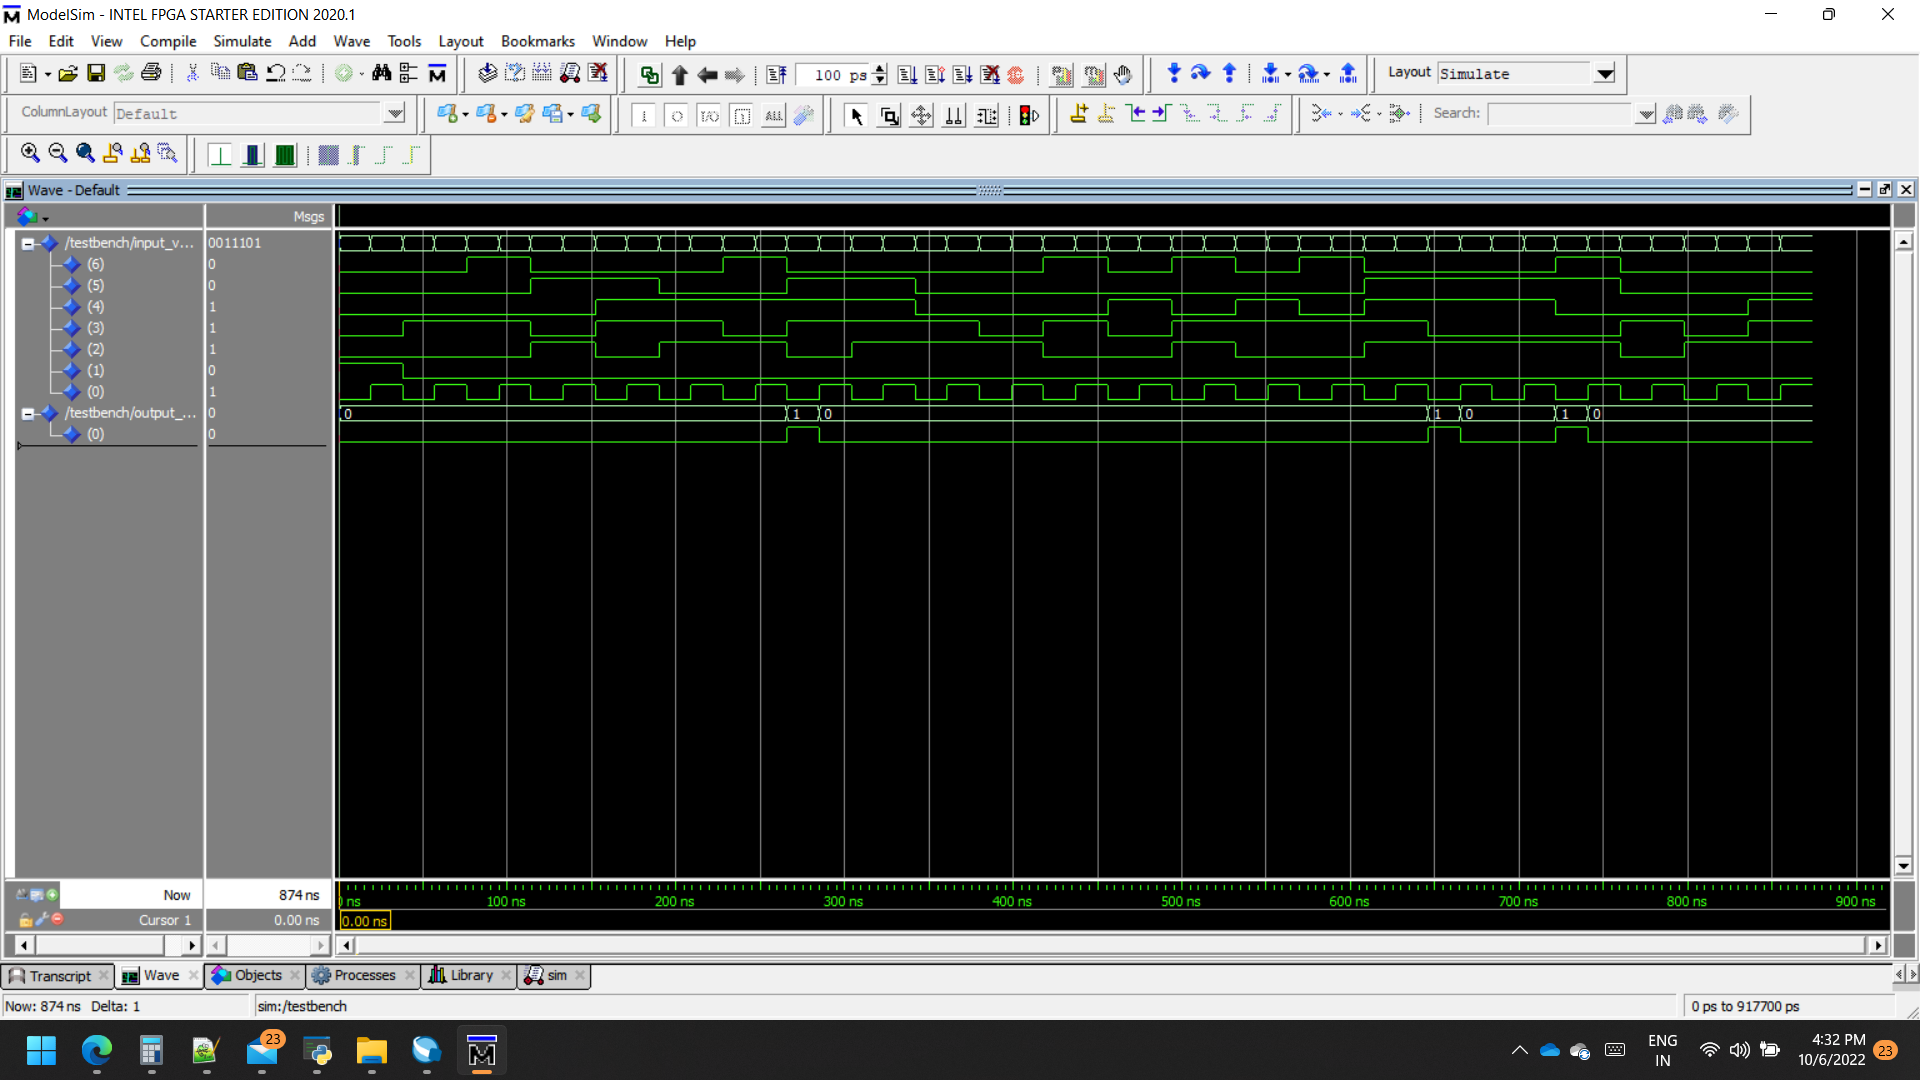
\includegraphics[width=\textwidth]{figs/strdet_waveform.PNG}  % change width to re-size the image.
	  % give a caption.
	  \caption{Waveform of the Multiple String Detector FSM}
	  % a label to refer to the figure
	  \label{fig:strdet_waveform}
	  
	\end{figure}
	
	\pagebreak
	Scanchain returned file from Xen10 board image for the Multiple String Detector
	\begin{figure}[H]
	  % will center the figure.
	  \centering
	  % include graphics (can include eps, jpg, pdf ...)
	  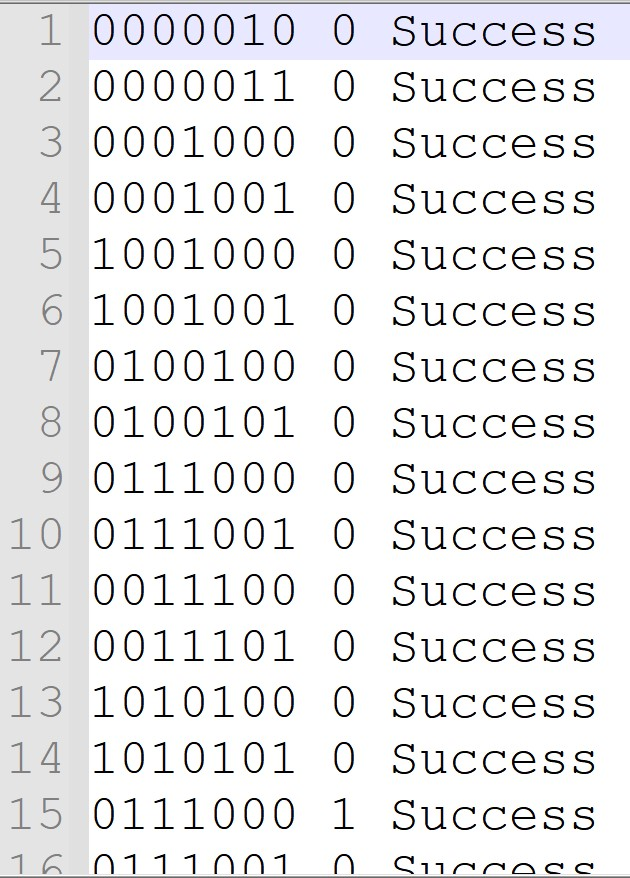
\includegraphics[width=0.6\textwidth]{figs/strdet_scan.JPG}  % change width to re-size the image.
	  % give a caption.
	  \caption{Scanchain success output of the Multiple String Detector FSM}
	  % a label to refer to the figure
	  \label{fig:strdet_scan}
	  
	\end{figure}
	
\end{document}
